\documentclass[12pt]{article}

\usepackage{indentfirst}
\usepackage[a4paper, total={6in, 8in}]{geometry}
\usepackage[singlespacing]{setspace}
\usepackage{fontspec}
\usepackage{graphicx}

\setmainfont{Times New Roman}

\title
{
	\textbf
	{
		SeeSharper
		\\
		Intuitive Drawing Application
		\\
		Documentation
	}
}

\author
{
	Baltariu Ionuț-Alexandru - 1305A
	\\
	Beldiman Vladislav - 1350A
	\\
	Nistor Paula-Alina - 1305B
	\\
	Rusu Iulian - 1305A
	\\
	\\
	\textit{"Gheorghe Asachi" Technical University of Iași}
	\\
	\textit{Faculty of Automatic Control and Computer Engineering}
} 

\date{}

\begin{document}

\maketitle 

\newpage

\clearpage
\vspace*{\fill}
\begin{center}
{\huge \textbf{Software Requirements Specification}}
\end{center}
\vfill 
\clearpage

\newpage
\tableofcontents
\newpage

\section{Introduction}
\subsection{Purpose}
The point of this document is to give a detailed description of the requirements for the SeeSharper application.
It will explain the purpose and features of the program, its interfaces and its core functionalities.

\subsection{Scope}
SeeSharper is a simple program that people can use for creating drawings and minimally editing images. The application must provide basic functionality for drawing and painting like different types of brushes, brush sizes and a color palette. 
SeeSharper should also provide shaped stencils and line tools, making the application useful for diagram development. After the drawing is ready, the user has the possibility to save the image in a specific format.

SeeSharper develops an efficiently easy to use interface. This application wants to be a simplified version of Microsoft Paint and Paint.Net.

\subsection{Overview}
The next chapter, the Overall Description section of this document, gives an overview of the functionality of the application. It describes expected user characteristics and general constraints. The third chapter, Specific Requirements section of this document, describes in technical terms the details of the functionality of the application and describes the graphical  user  interface.	

\section{Overall Description}
\subsection{Product Perspective}
SeeSharper is a stand-alone drawing application with minimal image editing capabilities written in C\# for the Windows Operating System. It aims to be an open source alternative to Microsoft Paint with a similar design and basic functionality unlike other open source products available such as GIMP.

SeeSharper will be implemented as a Windows Forms Application. The application will be developed with the Model-View-Presenter architecture, with a supervising controller. It will use a thread for the GUI and another one for the MVP components.
\subsection{Product Functions}
SeeSharper must provide the following major functions for its end users:
\begin{enumerate}
\item Image Loading - SeeSharper must be able to load user images so that they can be drawn on.
\item Drawing Saving - SeeSharper must have the functionality of saving a user drawing.
\item Customizable Brush - SeeSharper must provide a wide range of color selection, as well as different brush sizes.
\item Drawing Shapes - SeeSharper must provide easy to draw shapes with a customizable border and fill. 
\item Drawing Text - SeeSharper should provide a way to add text to the drawing.
\end{enumerate}
\subsection{User Classes and Characteristics}
SeeSharper is to be design for ease of use, especially for users that have not used a drawing application before. It, however, does not provide as many functionalities as a professional image editor in order to keep it from being overwhelming. Buttons and options should provide commonly used icons that convey their functionality instead of text or along with it whenever possible. Furthermore, menus should be easy to navigate without many layers of submenus. It is also designed for those who seek an open source application, but which is more accessible than its counterparts.
\subsection{Design and Implementation Constraints}
The main limiting constraints in this development cycle will be time as well as the technology constraint of developing everything for the .NET platform, which will be amplified by our inexperience with the C\# language, and inexperience in software design and documentation.

\section{Specific Requirements}
\subsection{External Interface Requirements}
\subsubsection{User Interfaces}
This section describes the graphical user interface (GUI) features and constraints.
\begin{enumerate}
\item The main window of the application should have a large canvas, initially with a white background.
\item A menu with options will be located in the top left corner (Load, Save, Help, etc.).
\item A menu that allows the user to select drawing tools.
\item When clicking the color menu, the user will see a new window where they will be able to select the desired RGB color. Optionally, other color spaces may be selectable.
\item Clicking on the Load/Save buttons will open a separate dialog window where the user will be able to open or save their drawing.
\item Clicking on the Help button will open a separate window with some documentation and/or tutorial.
\end{enumerate}

\subsubsection{Software Interfaces}
The application must provide a way to communicate with the underlying Operating System's API to delegate the saving/loading of drawings as image files. There are no other software interface constraints as the application is self-contained.
\subsection{Functional Requirements}
This section exemplifies the actual functionalities of the application, with in-depth information about every client observable feature.
\subsubsection{Color picking}
The user must be able to select the color in which to draw or represent a preselected geometrical form. Colors from all the RGB spectrum must be present in the application.
\subsubsection{Eraser tool}
The user must be able to use an eraser tool in order to delete previously done work in the drawing canvas. The size of the eraser should be user modifiable (within predefined bounds), improving performance when trying to remove large portions of a drawing.
\subsubsection{Brush tool(s)}
In order to paint properly, a brush-like took must be present in the application, that, when selected, gives the user the opportunity to draw any shape or object of the previously selected color and brush-size.

The application has to contain various types of brushes, of different dimensions and drawing styles, in order to give a pleasing and versatile end-user experience.

\subsubsection{Other advanced drawing tools}
\begin{enumerate}

\item  \textbf{Geometrical shape creator}

The user should be able to select a developer-defined geometrical shape and generate it on the canvas within wished bounds. Shapes must be defined by a number of points, usually two. Ideally, a preview of the shape being drawn should be displayed and modified in real time as the user drags the mouse on the canvas. After clicking to pick the final point on the canvas, the user should have the option to change the color of the shape by selecting a different color in the menu. At this point, the shape should also allow dragging with the mouse to translate its position on the canvas. Upon clicking again, the shape will be finalized and not modifiable anymore. Should the Undo option be available, it will completely remove the shape.

\item \textbf{Shape filling at drawing time}

The user might indicate if the shape that is to be drawn has to be filled with a color. If so, the fill color is a distinct one from the drawing color(border color) and can be selected from within the application.

\end{enumerate}

\subsubsection{Drawing saving/loading}

The application must offer the possibility of saving the current drawing to an image (of a selected extension) that will be located on the storage disk of the computer.

Similarly to the previously mentioned functionality, the application must offer the possibility of loading an already existing image that the user wishes to be modified.

\subsubsection{Undo/Redo}

In order to provide a rollback feature when making mistakes, the application must offer the possibility of undoing an action at any given point. It is also wished that any undone action can be redone.

These actions might be done either by pressing the corresponding buttons in the graphical user interface or by using the well known shortcuts: \textbf{CTRL+Z} for undo, and \textbf{CTRL+Y} for redo.

The user might even undo a previously loaded image, as it is permitted by the application.

If multiple undo actions are commited, and then the user draws something on the canvas, he might not redo any action that existed before the additional drawing element has been added to the canvas.

\subsubsection{Help window}

When clicking the 'Help' button, a window with all of the application's features will be provided to the user in the form of a .chm document. In this way, the typical user might research all of the tools and features that \textit{SeeSharper} is providing.

\subsection{Performance Requirements}
This section covers the requirements that concern the performance of the application in response to user interaction. It is aimed to describe general use case scenarios, as well as time performance constraints.
\begin{enumerate}
\item \textbf{Usage of the toolbar menu}
\\
The graphical interface must provide a menu that must be easily accessed at the top of the main application window in one click.
\item \textbf{Usage of drawing tools}
\\
All drawing tools must be easily selectable from a unified menu of drawing tools. The user should have the option to change the color, size and any other parameters of a selected tool easily.
\item \textbf{The drawing process}
\\
Drawing must feel smooth and be responsive to user input. The application should provide a way to undo/redo changes from history, without noticeably slowing down performance.
\item \textbf{File system interaction}
\\
All drawings must have the ability to be saved on the disk in a specific image format (\texttt{png, jpeg, bmp}). The application should provide a way to load images into the canvas and draw on them. The process of saving and loading should not take longer than doing so in other applications that interact with the file system.
\item \textbf{General timing constraints}
\\
Any user input should be processed without a noticeable delay. In the event that a more complex computation is required, the user must be notified and the graphical interface must remain responsive for the whole duration. Additionally, the interface may provide status messages to notify the user.
\end{enumerate}

\subsection{Design Constraints}
This section describes the limitations imposed on the application by software or hardware characteristics of the environment.
\begin{enumerate}
\item \textbf{Disk space usage}
\\
The whole application must not occupy more than 20 MB of disk storage.
Ideally, the application should fit into 10 MB.
\item \textbf{Memory usage}
\\
The application's RAM usage must not exceed 15 MB.
Ideally, the application should not use more than 8 MB of RAM.
\end{enumerate}

\subsection{Attributes}
This section describes different software system attributes, metrics and requirements for them.
\begin{enumerate}
\item \textbf{ System reliability}
\\
Reliability refers to the system's capacity to correctly respond to user input.
The application must correctly load, save and draw images 100\% of the time.
\item \textbf{Maintainability}
\\
The application should be easily maintainable and extendable.
The code should allow easy testing and should be open for future extensions and new features. 
\end{enumerate}

\clearpage
\vspace*{\fill}
\begin{center}
{\huge \textbf{UML Diagrams}}
\end{center}
\vfill 
\clearpage

\clearpage
\vspace*{\fill}
\begin{center}
\setcounter{page}{15}
{\huge \textbf{How to use the application}}
\end{center}
\vfill 
\clearpage

\section*{Drawing lines or various geometric shapes}

In order to draw lines (straight or curved) or other shapes, the user has to select the shape before actually drawing on the canvas.

Keep in mind that in order to draw geometric shapes, the \textbf{click} mouse button has to be hold, then drag the figure to respect wished dimensions.

\begin{figure}[h]
\centering
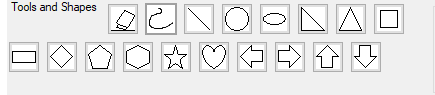
\includegraphics[width=10.5cm]{graphics/tools_and_shapes.png}
\caption{Tools and shapes menu}
\end{figure}

\begin{figure}[h]
\centering
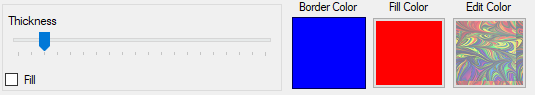
\includegraphics[width=10.5cm]{graphics/thickness_fill_colors.png}
\caption{Tools and shapes menu}
\end{figure}

The user can also select whether the shape that is to be drawn will be filled by checking the "Fill" box in \textbf{Figure 2} and might also change the border line thickness by dragging slider bar.

\section*{Changing drawing colors}

As seen in \textbf{Figure 2}, the user can changed both the \textit{fill} and \textit{border} colors.  

Firstly, the user has to select whether he wants to change the fill or the border colors, then, the \textbf{Edit Color} button has to be pressed. The following window will appear:

\begin{figure}[h]
\centering
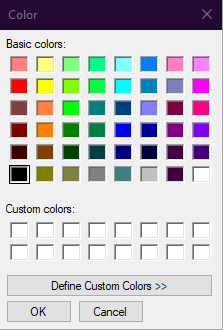
\includegraphics[width=2.5cm]{graphics/colors.png}
\end{figure}

Here, any given color can be selected. However, if the user wants to select a custom color, the \textbf{Define Custom Colors >>} button has to be pressed.

After that, one can give custom wanted colors by either entering RGB color codes or by selecting one from the window on the right.

\begin{figure}[h]
\centering
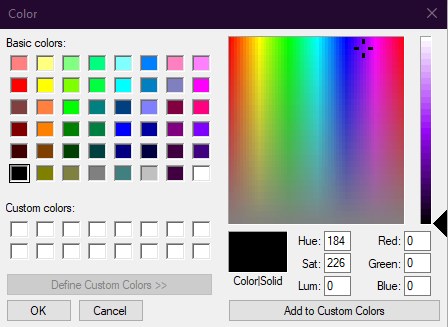
\includegraphics[width=4.5cm]{graphics/custom_colors.png}
\caption{Custom color selection}
\end{figure}

\section*{Erasing}

From \textbf{Figure 1} select the \textit{Eraser tool} (the first square in line), change the thickness depending on the size of the area that is to be erased and, finally, erase by holding the click button on the canvas.

\section*{Using undo/redo functionality}

After drawing a shape, if the user considers that a mistake has been made, he might undo the latest actions by clicking the \textbf{Undo} button \textbf{(Figure 4)}.

\begin{figure}[h]
\centering
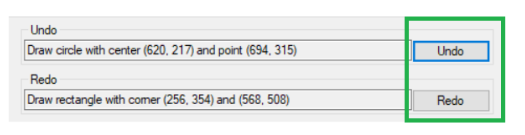
\includegraphics[width=9.5cm]{graphics/undo_redo.png}
\caption{Undo/Redo buttons}
\end{figure}

If mistakes have been done while undoing, there is also the possibility to redo previously undone actions by pressing the \textbf{Redo} button. \textbf{(Figure 4)}


\section*{Saving/loading drawings/images}

The application allows both loading and saving an image or a drawing to the file system as a PNG file. \textbf{(Figure 5)}

\begin{figure}[h]
\centering
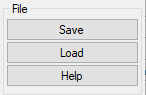
\includegraphics[width=5.5cm]{graphics/save_load_help.png}
\caption{Menu for saving/loading}
\end{figure}

After clicking the \textbf{Save} button, the user has to navigate to the wished saving location and then give a valid name to the file, ending by clicking again the \textbf{Save} button in the new window.

\begin{figure}[h]
\centering
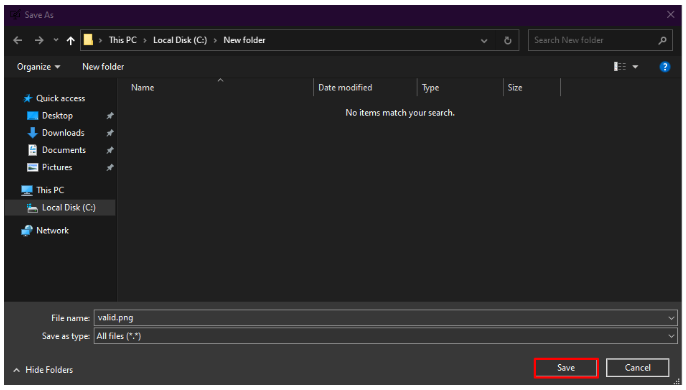
\includegraphics[width=11.5cm]{graphics/save.png}
\caption{Save window}
\end{figure}

Same principles apply to the \textbf{Load} functionality.

\section*{Accesing help from within de application}

Navigate to the menu at \textbf{Figure 5}, then click the \textbf{Help} button.

After that, use the menu found on the left side of the window to access information about wanted subjects.

\begin{figure}[h]
\centering
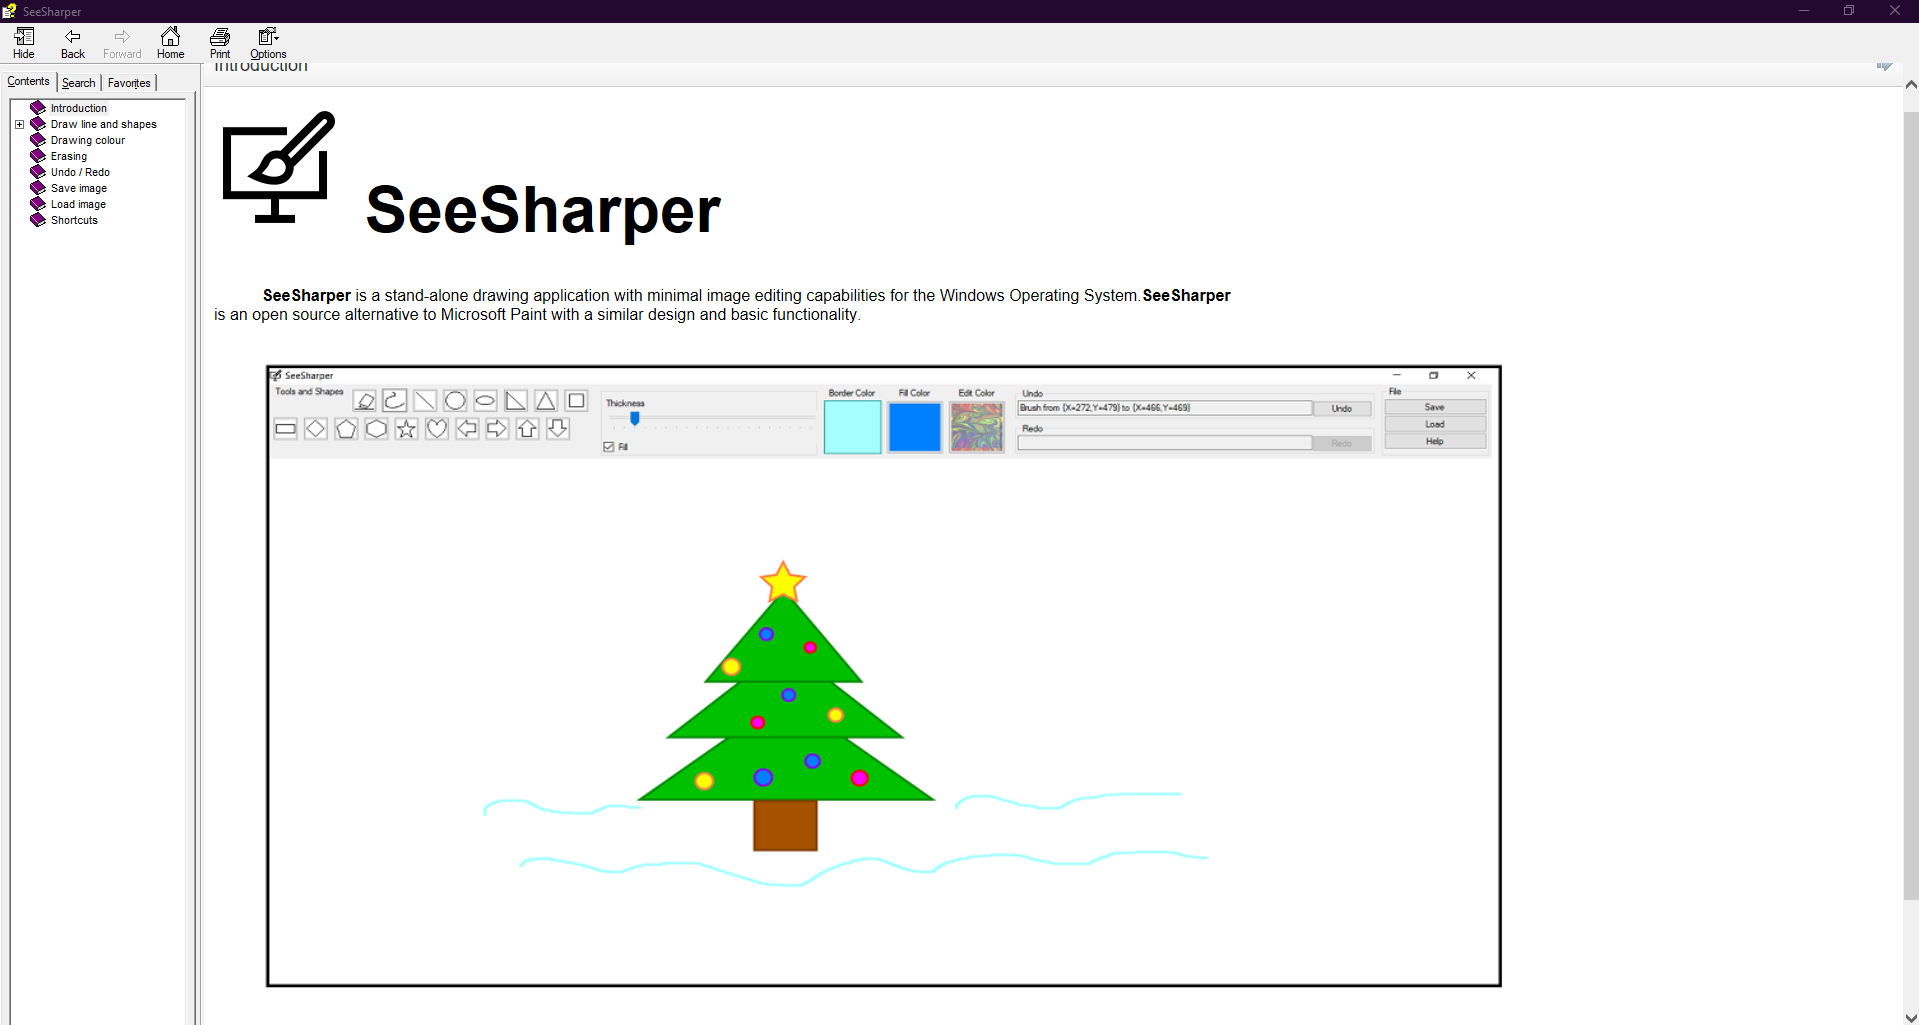
\includegraphics[width=13.5cm]{graphics/help.png}
\caption{Help window}
\end{figure}

\section*{Shortcuts}

\begin{center}
\begin{tabular}{ |c|c|} 
 \hline
 \textbf{Shortcut} & \textbf{Action} \\ 
  \hline
 CTRL+S & Save \\ 
  \hline
 CTRL+L & Load \\ 
 \hline
 CTRL+H & Open Help  \\ 
  \hline
 CTRL+Z & Undo \\
  \hline
 CTRL+Y & Redo \\
  \hline
\end{tabular}
\end{center}

\clearpage
\vspace*{\fill}
\begin{center}
{\huge \textbf{Screenshots of the application}}
\end{center}
\vfill 
\clearpage

\begin{figure}[h]
\centering
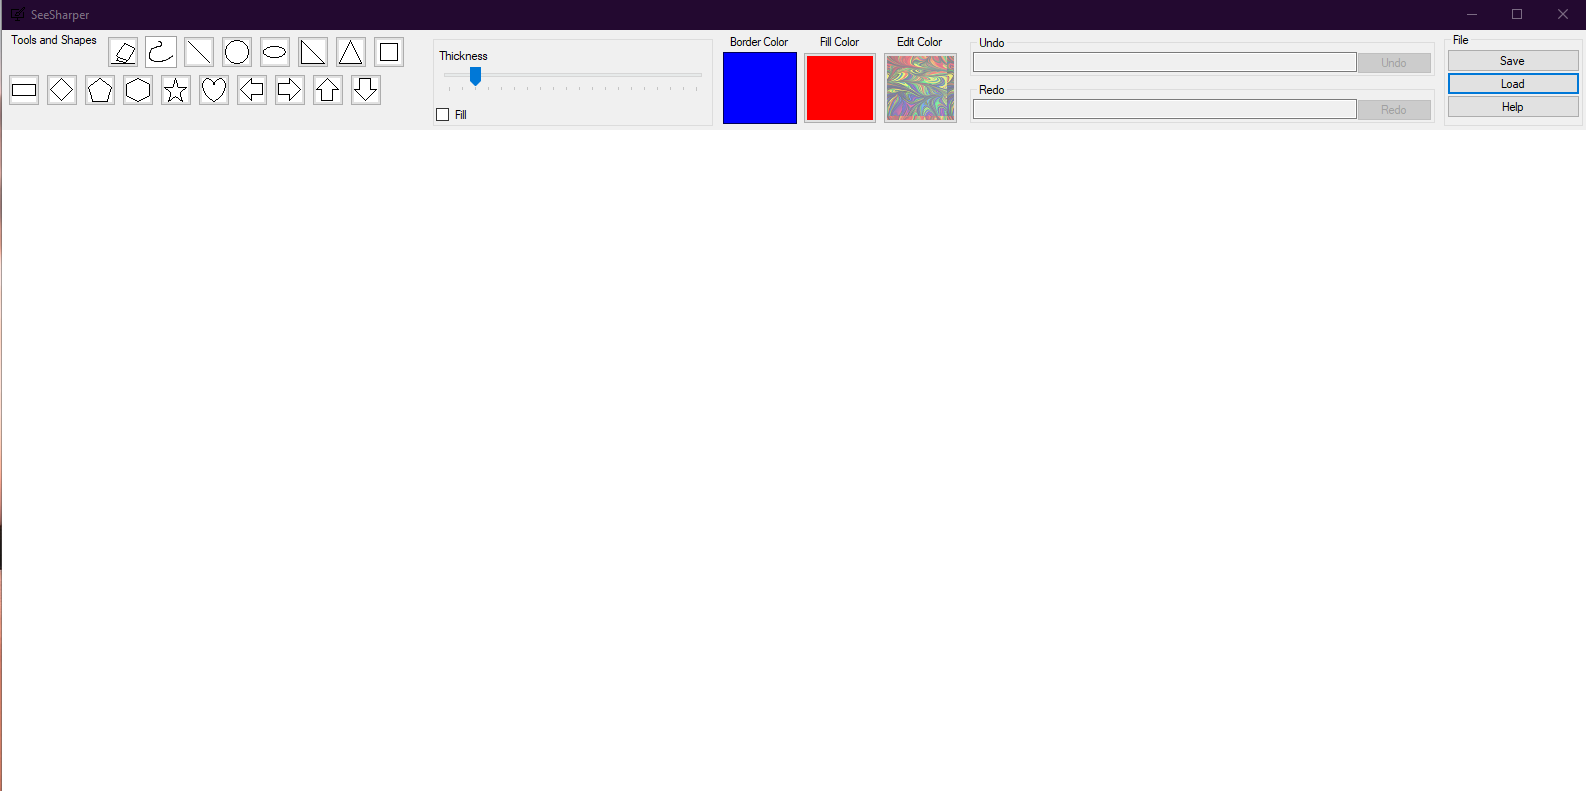
\includegraphics[width=11.5cm]{graphics/seesharper_empty.png}
\caption{Application at start}

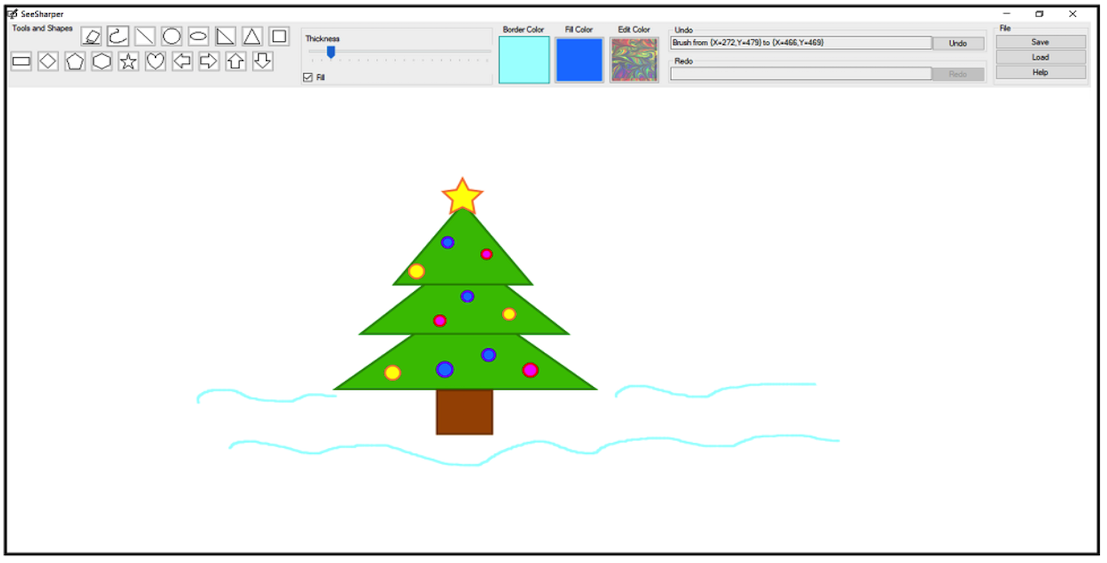
\includegraphics[width=11.5cm]{graphics/seesharper_drawing.png}
\caption{Application after drawing}

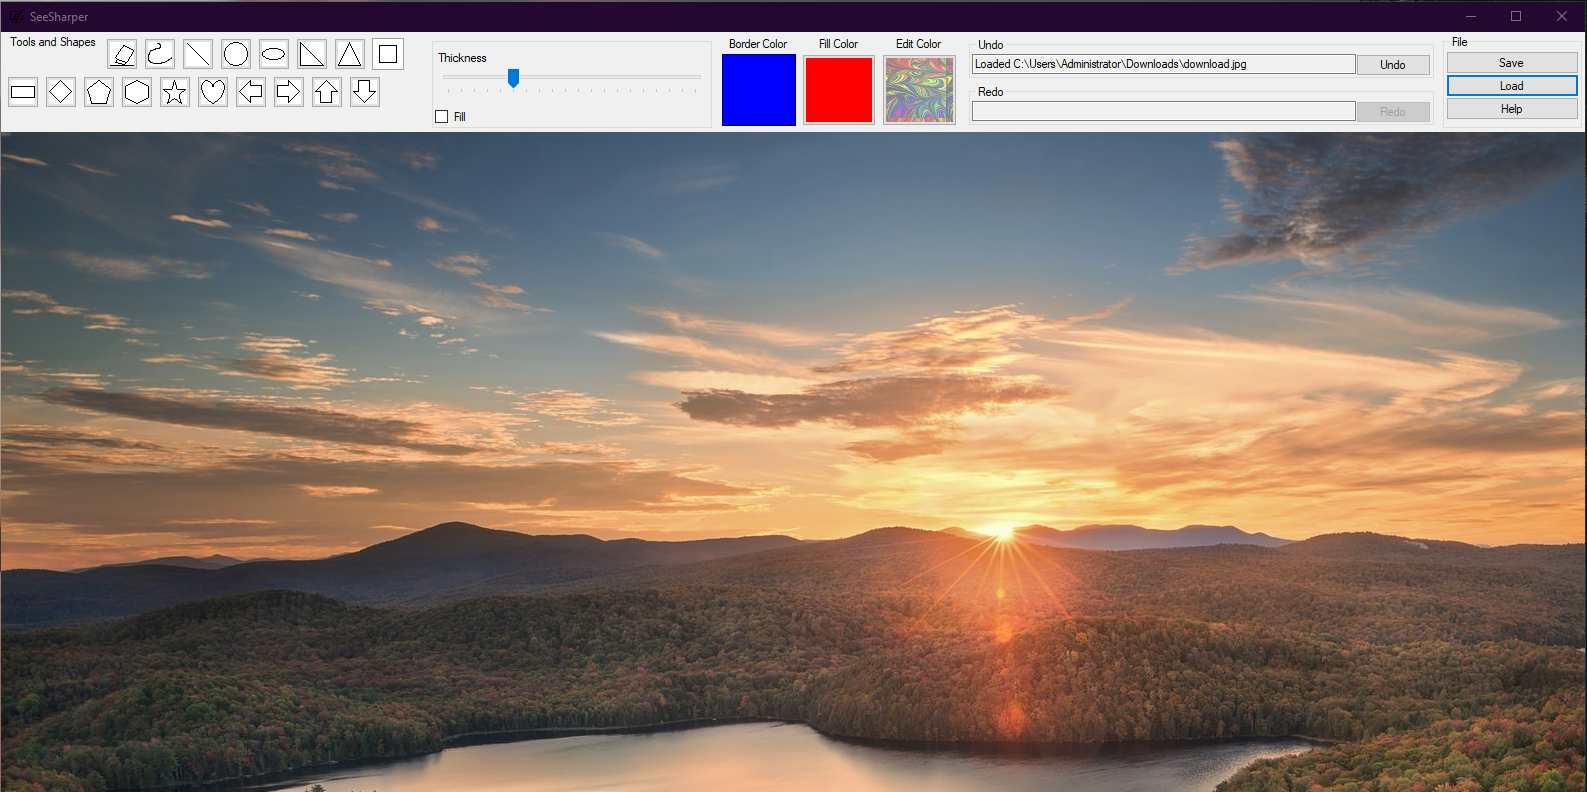
\includegraphics[width=11.5cm]{graphics/loaded_img.png}
\caption{Application after loading an image}

\textit{More screenshots can be seen at the previous section.}
\end{figure}


\end{document}
